\documentclass{suturo}

\begin{document}
    \maketitle{Planning}{02.01.2017}{}{1}{}{}{}{}

\makeatletter
\newcommand{\chapterauthor}[1]{%
  {\parindent0pt\vspace*{-27pt}%
  \linespread{0}\small\begin{flushright}von: #1\end{flushright}%
  \par\nobreak\vspace*{0pt}}
  \@afterheading%
}
\makeatother

\section{Node: main (planning\_main\_programm)}
\subsection{Architekturbild}
\chapterauthor{Kevin Störmer}
\begin{center} 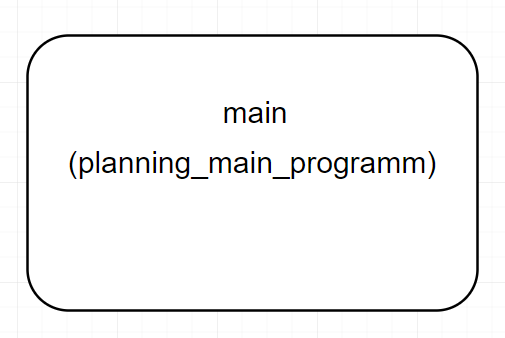
\includegraphics[width=0.4\textwidth]{img/diag_planning_main_programm.png} \end{center}
\subsection{Beschreibung des Teilsystems}
\subsubsection{\"Ubersicht}
\chapterauthor{Kevin Störmer}
Die Node 'main' im Paket 'planning\_main\_programm' soll ausschliesslich auf höchster Ebene den internen Ablauf des PR2 modellieren. Dabei wird der folgende Ablauf sequenziell ausgef\"uhrt:\\
(TOLLES SCHAUBILD)\\ \\
Alle dafür notwendigen Logiken, die auf Basis externer Daten entschieden werden, wurden dabei basierend auf der Quelle der Daten in andere Nodes ausgelagert. Dabei wurde z.b der Vergleich zweier Punkte aus Vision in die Node 'points' (Paket: planning\_vision) ausgelagert.

\section{Node: points (planning\_vision)}
\subsection{Architekturbild}
\chapterauthor{Kevin Störmer}
\begin{center} 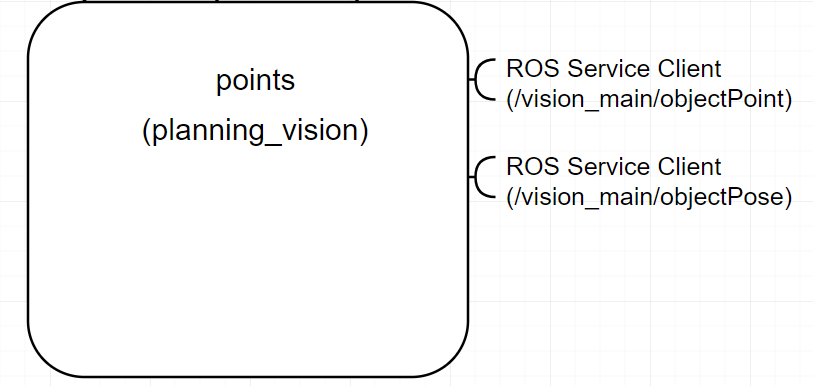
\includegraphics[width=0.6\textwidth]{img/diag_planning_vision.png} \end{center}
\subsection{API}
\chapterauthor{Kevin Störmer}
\subsubsection{Serviceclients}
1. '/vision\_main/objectPoint' \\
Nimmt Objekt über Kinect wahr, und gibt Mittelpunkt des Objektes zur\"uck.\\ \\
2. '/vision\_main/objectPose' \\
Nimmt Pose (steht oder liegt) des Objektes wahr.
\subsection{Beschreibung des Teilsystems}
\subsubsection{\"Ubersicht}
\chapterauthor{Kevin Störmer}
Die Node 'points' aus dem Paket 'planning\_vision' befasst sich ausschliesslich mit der Kommunikation mit Gruppe-Vision und Logiken auf Basis der wahrgenommenen Daten. Dabei werden Services zur Position und Pose des Objectes in Anspruch genommen und ausgewerten. Zudem wird eine Methode zur Validierung zweier Punkte angeboten.

\section{Node: ask (planning\_knowledge)}
\subsection{Architekturbild}
\chapterauthor{Kevin Störmer}
\begin{center} 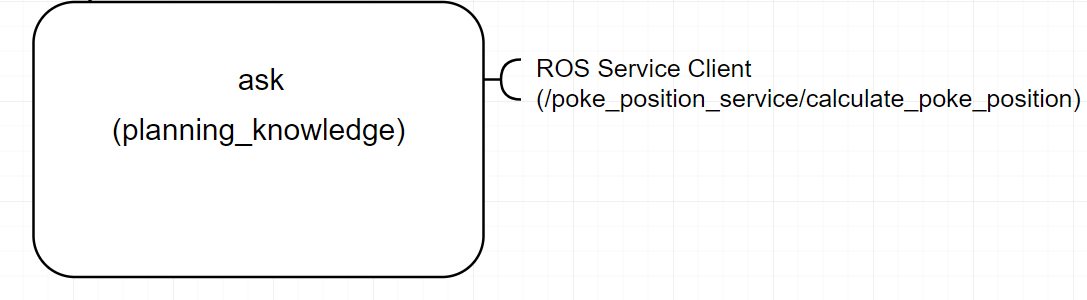
\includegraphics[width=0.8\textwidth]{img/diag_planning_knowledge.png} \end{center}
\subsection{API}
\chapterauthor{Kevin Störmer}
\subsubsection{Serviceclients}
1. '/poke\_position\_service/calculation\_poke\_position' \\
Berechnet den zu stupsenden Punkt des Objektes
\subsection{Beschreibung des Teilsystems}
\subsubsection{\"Ubersicht}
\chapterauthor{Kevin Störmer}
Die Node 'ask' im Paket 'planning\_knowledge' ist ausschliesslich für die Kommunikation mit Gruppe Knowledge zust\"andig.

\section{Node: actions (planning\_motion}
\subsection{Architekturbild}
\chapterauthor{Kevin Störmer}
\begin{center} 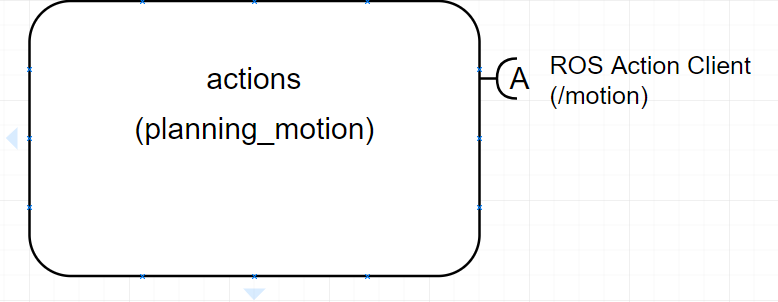
\includegraphics[width=0.6\textwidth]{img/diag_planning_motion.png} \end{center}
\subsection{API}
\chapterauthor{Kevin Störmer}
\subsubsection{Actionclients}
1. '/motion' \\
Bewegt die Arme des Pr2 entweder in die Home-Position oder zu einem bestimmten Punkt.
\subsection{Beschreibung des Teilsystems}
\subsubsection{\"Ubersicht}
\chapterauthor{Kevin Störmer}
Die Node 'actions' im Paket 'planning\_motion'  ist ausschliesslich für die Kommunikation mit Gruppe Motion zuständig. Dabei wird die Action '/motion' einmal für die Home-Position des Pr2 und zum Bewegen des Armes zu einem bestimmten Punkt genutzt.

\section{Node: movement (planning\_move)}
\subsection{Architekturbild}
\chapterauthor{Kevin Störmer}
\begin{center} 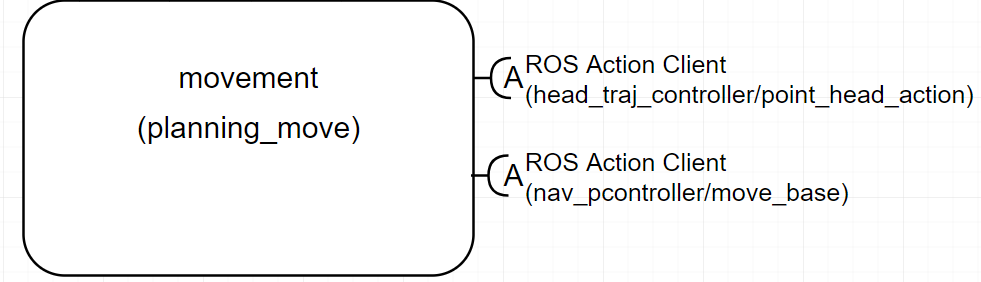
\includegraphics[width=0.8\textwidth]{img/diag_planning_move.png} \end{center}
\subsection{API}
\chapterauthor{Kevin Störmer}
\subsubsection{Actionclients}
1. 'head\_traj\_controller/point\_head\_action' \\
Bewegt den Kopf des Pr2 in Richtung eines Punktes.\\ \\
2. 'nav\_pcontroller/move\_base' \\
Bewegt die Basis des Pr2 in Richtung eines Punktes.
\subsection{Beschreibung des Teilsystems}
\subsubsection{\"Ubersicht}
\chapterauthor{Kevin Störmer}
Die Node 'movement' im Paket 'planning\_move' behandelt alle Fälle in denen sich der Pr2 bewegen soll, welche nicht von Gruppe Motion abgehandelt werden. Dabei eine Methode zum Bewegen des Kopfes des Pr2 angeboten sowie eine Methode zum Bewegen der Basis des Pr2.


\end{document}
